\section{Force calculation}

\begin{frame}
    \frametitle{$F_{ij} = -F_{ji}$}

    \begin{columns}
        \begin{column}{0.5\textwidth}
            \textbf{Task:} Implement Force calculation with the pairwise iterator

            \textbf{Solution:} Skip repeating calculations due to $F_{ij} = -F_{ji}$
            \begin{equation}
                F_i = \sum_{j=1, j \neq i}^{\#particles} F_{i,j}
            \end{equation}
            \begin{align}
                F_{i,j} &= \frac{m_im_j}{(||x_i-x_j||_2)^3} (x_j - x_i) \\
                        &= \frac{m_jm_i}{(||x_j-x_i||_2)^3} \left(-1 \cdot \left(x_i - x_j\right)\right) \\
                        &= - F_{j,i}
            \end{align}
        \end{column}
        \begin{column}{0.5\textwidth}
            \begin{figure}[]
                \centering
                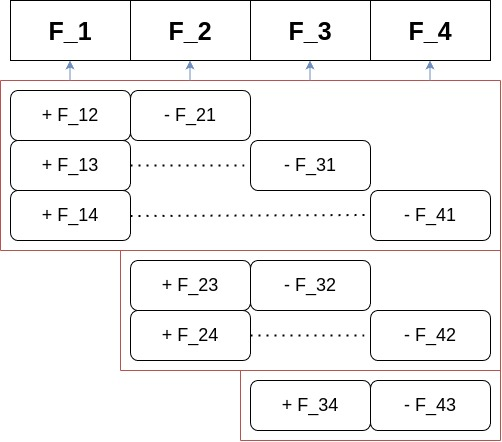
\includegraphics[width=\columnwidth]{ForceCalcFig.jpg}
                \caption{Force calculation}
            \end{figure}
        \end{column}
    \end{columns}

    
\end{frame}